\appendix
\chapter{}
\addcontentsline{toc}{chapter}{Anhang A}\label{anhangA}

\textbf{Affinitätsdiagramm}:

\begin{figure}[H]
	\centering
	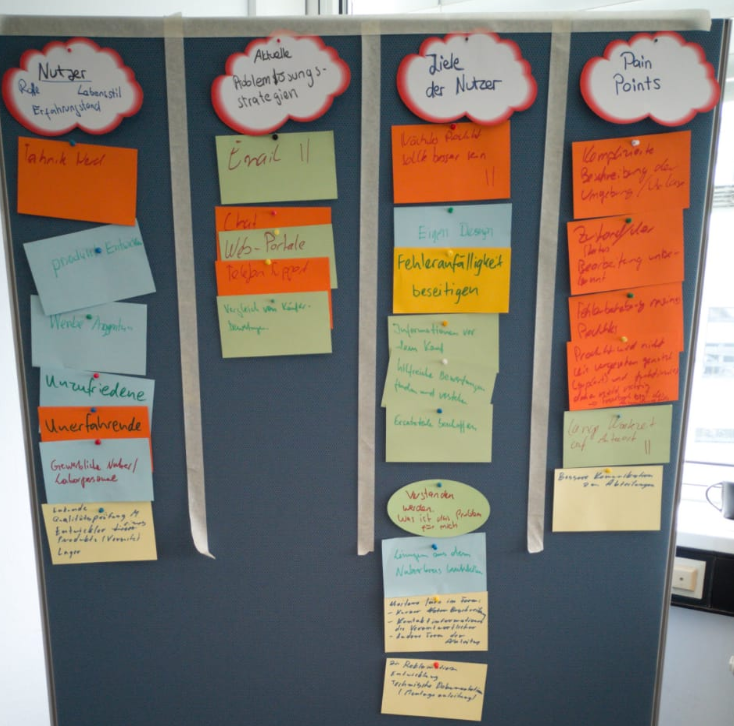
\includegraphics[width=0.50\textwidth]{resources/anhang/Affinitaetsdiagramm.png}
	\caption{Das im Kreativ Workshop am 03.05.2019 entstandene Affinitätsdiagramm welches als Grundlage für die Erstellung von Personas diente. Quelle: Eigene Darstellung}
	\label{img:affinitydiagramm}
\end{figure}

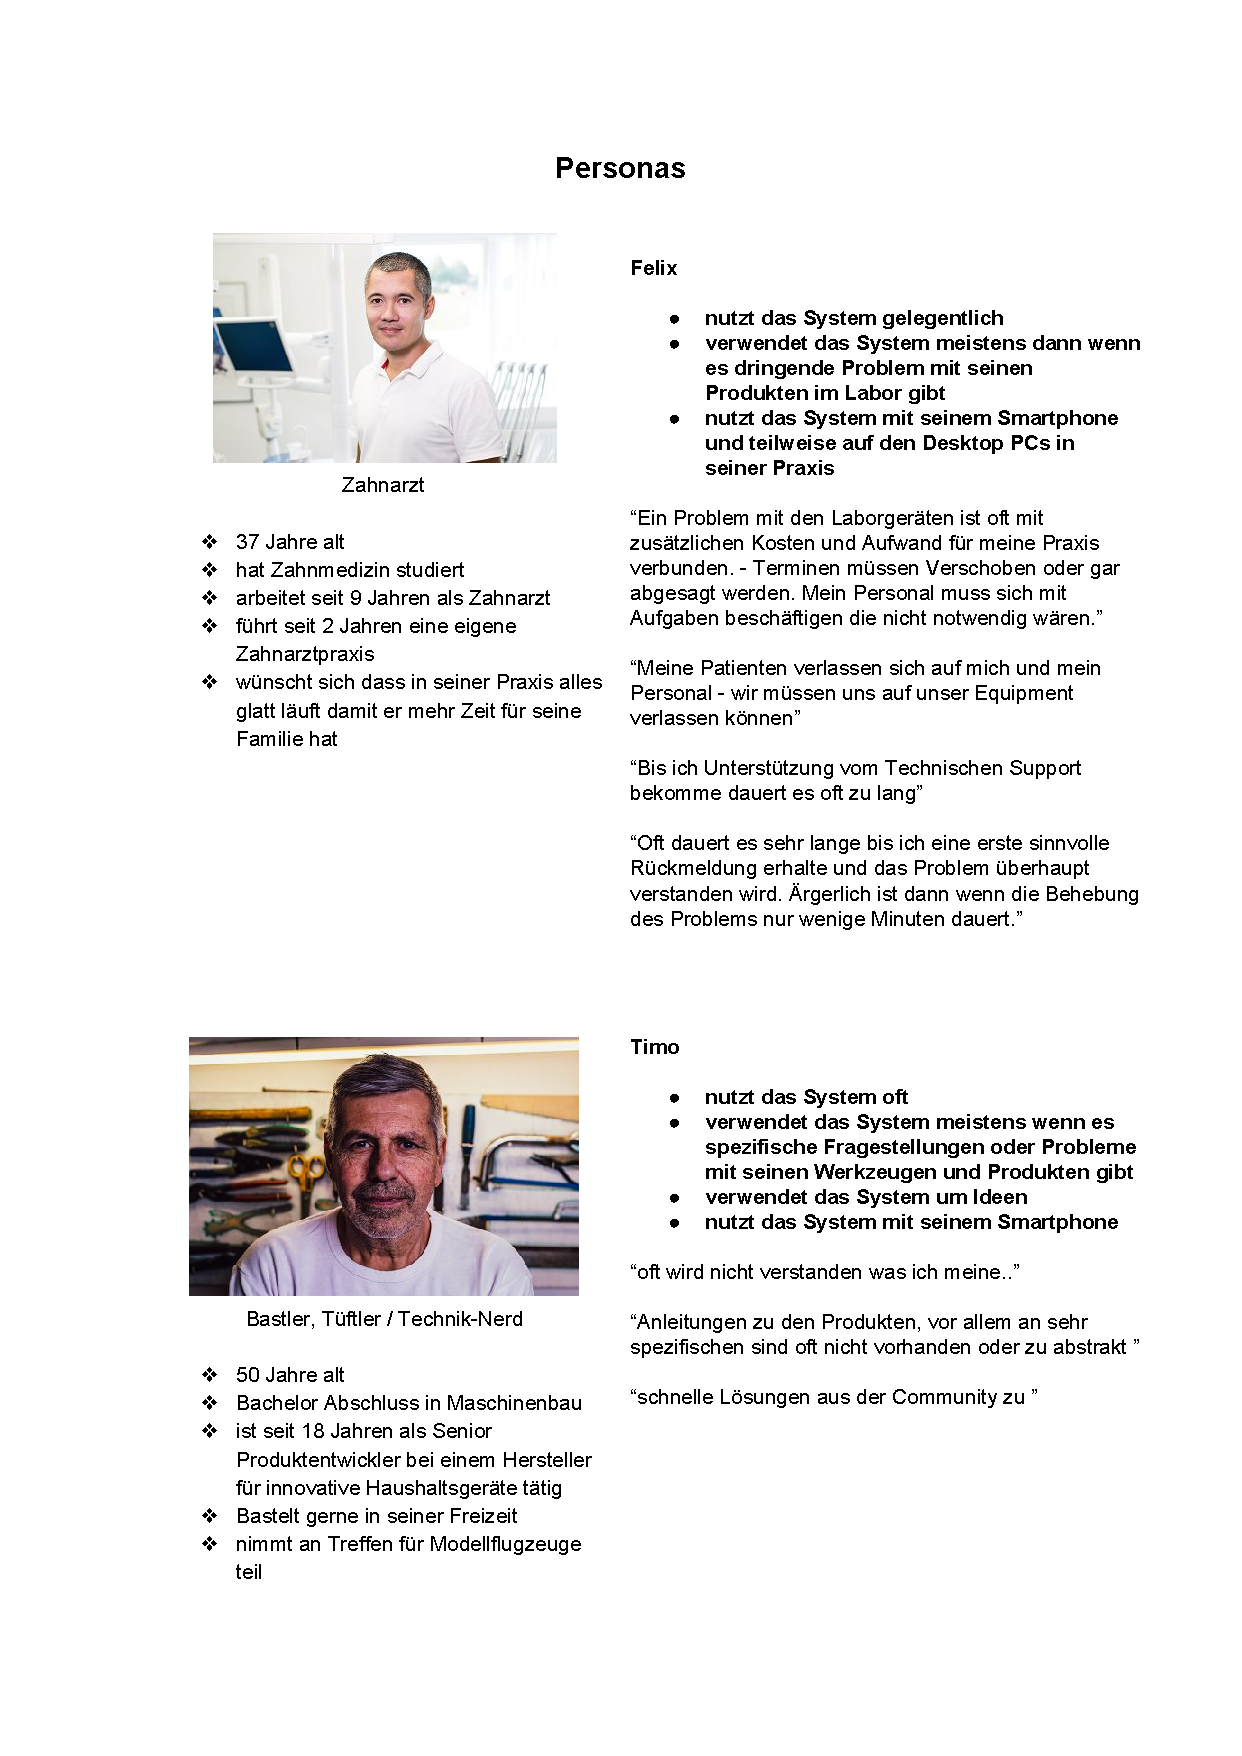
\includepdf[pages=-]{resources/anhang/Personas.pdf}

\addcontentsline{toc}{chapter}{Szenarien}

\textbf{Ist-Szenarien}

\textbf{Felix}

Am Dienstagabend nach der Sprechstunde, entscheidet sich Felix, dem technischen Support des
Herstellers für die Beleuchtungsanlage im Behandlungsraum A, eine E-Mail zu schreiben. Denn die
Leuchte bleibt nicht stabil in seiner Ausrichtung sondern rutscht immer wieder seitlich nach runter.
Nicht nur er ist darüber sehr verärgert sondern auch seine Arzthelferin. Diese muss bei Eingriffen, bei
welchen, Felix eine gute Ausrichtung der Beleuchtung besonders wichtig ist, die Leuchte immer
wieder richtig ausrichten. An manchen Eingriffen ist sie sogar nur noch damit beschäftigt. Er hatte die
Anfrage im Support bereits vor eineinhalb Wochen geöffnet, doch nach der ersten Rückmeldung
folgte nur ein E-Mail Ping-Pong mit Gegenfragen wurden und Vorschläge die er ausprobieren sollte,
jedoch nicht geholfen haben.
Am Mittwochnachmittag erhält Felix eine Antwort. Der Hersteller reagiert diesmal mit dem Angebot
einer Skype-Session. Vier Experten werfen an diesem Videoanruf einen Blick auf die Leuchte und
tauschen sich aus untereinander aus. Einer von diesen wurde, spontan noch dazu gerufen. Nach
kurzer Zeit stellt sich heraus dass an dem Modell welches bei Felix im Praxis in Einsatz ist, ein
Gelenk angebracht ist, welches ein sehr seltenes Exemplar ist. Einem der Support Ingenieure der
dieses Modell zufällig einmal bei einem Kunden im Einsatz gesehen hatte, fällt ein, dass bei diesem
Modell, am Drehgelenk, eines der M6er Schrauben mit einer M7er Schraube ausgetauscht werden
musste, um das Gelenk stabiler zu machen. Der Hersteller schickt daraufhin einen Techniker, und die
Schraube wird ausgetauscht. Felix ist nun besonders verärgert da ein Problem welches in fünf
Minuten behoben werden konnte, ihm und seiner Personal sehr viel Wertvolle Zeit und Mühe gekostet
hat. Die Entschuldigungen des des technischen Supports über den Verlauf dieser Anfrage und die
Beteuerungen diesen Sachverhalt an das Produktmanagement und an das Doku-Team für die
weitere Aufarbeitung weiterzugeben besänftigen seine Verärgerung kaum.

\vspace{2mm}
\textbf{Timo}

Timo freut sich. Es ist endlich Samstag, seine Freundin ist auf Junggesellinnenabschied und er hat
endlich wieder Zeit an seinen Modellfliegern zu werkeln. In drei Wochen findet ein Treffen der
Modellflieger Community am Nachbarort statt und er will seine Flieger bis dahin auf Vordermann
bringen. Vor einigen Wochen hatte er bereits angefangen, sich um das etwas kränklich anhörende
Motor, eines seines seiner Flieger zu kümmern. Vor zwei Wochen hatte er hierzu eine Frage im
Forum “Modellfliegerprofis.de” gepostet und gefragt ob jemand eine Ahnung hätte, ob für die M16er
Schraube links neben der Lötstelle des Einlassventils eine Mutter von einem anderen Hersteller
verwendet werden kann? Ob da schon einmal jemand eine andere Mutter ausprobiert hat und ob dies
geholfen hat.
Er hat wenig Hoffnung dass jemand sinnvoll auf seine Frage antworten konnte, dennoch wirft er mal
einen Blick in das Forum. Wie erwartet haben nur wenige auf seine Frage reagiert und die meisten
haben nicht genau verstanden worum es geht. Er beantwortet noch einige Fragen und schließt etwas
frustriert das Forum.
Drei Wochen später am Treffen der Modellflieger hat er dann die Gelegenheit sein Anliegen den
anderen Technikaffinen direkt am Modell zu zeigen und sich über seine Frage auszutauschen. Es
stellt sich heraus dass, einige den Blog Beitrag gesehen haben, sich jedoch gar nicht erst die Mühe
gemacht haben die betreffende Stelle am Flieger anzuschauen. Vielen geht aus seiner Beschreibung
nicht klar hervor welche Stelle am Flieger er genau meint. Links neben des Einlassventils gebe es
mehrere Lötstellen. Einigen war die Beschreibung zu kompliziert und wussten gar nicht wie eine
M16er Schraube überhaupt aussieht.
Für Timo ist es nicht neu, dass dieser Art von Fragen und Antworten am Ort und Stelle am Modell viel
einfacher beschrieben, diskutiert und oft auch Lösungen gefunden werden können.


\vspace{2mm}
\textbf{Svenja}

Svenja ist fix und alle! Es ist Mittwochabend, sie hat gerade ihr Fitness Workout hinter sich gebracht
und wartet in Ihrem Lieblingskaffee auf ihren Kumpel Timo. Der hat ihr geschrieben dass er sich
etwas verspäten wird.
Svenja hört während des Workouts oder auch in der Agentur während der Arbeit gerne Musik und hat
sich vor kurzem neue Bluetooth Kopfhörer gegönnt. Die Kopfhörer sehen sehr hochwertig aus und
gefallen ihr vor allem wegen der schönen Gestaltung. Außer die etwas nach ihrer Meinung zu
auffällige Rille an einer bestimmten Stelle des Aufbewahrungsbox der Kopfhörer. Sie hat eine Menge
für diese Kopfhörer investiert. Fast ein Drittel ihrer Ausbildungsvergütung.
Sie hatte sich vorgenommen, Feedback zu diesem Produkt abzugeben. Da sich Timo nun verspäten
wird, entschließt sie sich, die Zeit zu nutzen um das zu erledigen. Sie hat gesehen dass in dem
Onlineshop in dem sie die Kopfhörer gekauft hat, Rezessionen geschrieben werden können. Sie holt
sich ihr Handy raus, loggt sich im Onlineshop ein und sucht sich die Kopfhörer in ihren letzten
Bestellungen heraus. Sie hatte zuvor noch nie eine Rezension geschrieben, doch nach etwas hin und
her klicken gelangt sie zu einem Formular wo sie Eingaben machen kann. Es werden ihr einige
Kriterien vorgeschlagen, welche Sie an dem Produkt bewerten kann (z. Bsp. die Soundqualität,
Gestaltung usw.). Das findet sie praktisch. Sie gibt für die Gestaltung 4 Sterne. Doch sie findet dass in
diesem Fall, eine Begründung für den Stern Abzug sehr angebracht wäre. Sie versucht die Stelle zu
beschreiben, doch in dem Moment fällt ihr auf, das dies eigentlich gar nicht so einfach ist. Besser
wäre wenn sie von der Stelle ein Bild machen und mit einer Bildbearbeitungsprogramm markieren
würde (so ein Programm ist sowieso standardmäßig auf ihrem Handy installiert denkt sie sich.).
Dennoch findet sie das jetzt etwas aufwendig. Im Augenwinkel sieht sie auch schon den Timo aus
dem Tram aussteigen und in ihre Richtung zu laufen. Sie schließt den Browser und nimmt sich das für
ein anderes mal vor.


\textbf{Soll-Szenarien}


\textbf{Felix}

Es ist Donnerstagnachmittag, Felix hat Mittagspause und kommt gerade vom Mittagessen. Am
Mittagessen haben Felix und Gül (seine Arzthelferin) sich über die Beleuchtungsanlage im
Behandlungsraum A unterhalten. Gül beklagt sich dass dieser so oft nicht in der ausgerichteten
Position bleibt und immer wieder nach unten rutscht.
Felix entschließt sich mit dem technischen Support des Herstellers Kontakt aufzunehmen. Er erinnert
sich noch, dass er vor einigen Wochen eine E-Mail von diesen erhalten hatte worin ein neues
Feedback Feature beworben wird. Man könne damit Feedback direkt am Produkt abgeben. Er findet
schnell diese E-Mail und erkundigt sich über das Feature. Es hört sich ganz gut dafür
geeignet zu sein um über die Leuchte ein Feedback abzugeben. Er ist jedoch etwas skeptisch. Er lädt
die vom Hersteller beschriebene App herunter und gibt einige Daten wie zum Beispiel seine Kundennummer ein.
Im App findet er eine Auflistung von Produkten die er von diesem Hersteller in seiner Praxist hat. 
Er wählt aus dieser Auflistung die Leuchte. Daraufhin erscheint ein Bildschirm auf welches er angeben soll um
welcher Kategorie sein Feedback eingeordnet werden soll: Es ist die Kategorie “Gestaltung” vorausgewählt. 
Er schaut sich die anderen Kategorien an und, wählt “Beeinträchtigung in der Nutzung” aus.

Nachdem er auf das Button “Fortfahren” geklickt hat, schaltet sich die Kamera seines Smartphones
ein und in halbtransparenter Schrift wird er aufgefordert, die Kamera auf die Leuchte zu richten. 
In dem Moment wo er die Leuchte durch das Display seines Smartphones sieht, wird die Leuchte auf dem
Bildschirm seines Smartphones mit einer virtuellen, halbtransparenten, gräulichen Silhouette umhüllt. 
Es erscheint nun in der Mitte des Bildschirms, ein Art Fadenkreuz in einem Ring.
Felix soll nun die Kamera nah auf das Teil am Produkt richten, für das er ein Feedback abgeben
möchte und zweimal auf das Fadenkreuz tippen um es auszuwählen. Dies wird ihm auf dem Bildschirm in 
halbtransparenter Schrift unter dem Ring mit dem Fadenkreuz eingeblendet.
Also bewegt Felix die Kamera in Richtung des Gelenks welches immer wieder herunterrutscht. Während
er die Kamera in Richtung des Gelenks bewegt färbt sich jeweils das Teil am Produkt welches sich
dem Mittelpunkt der Kamera am nächsten befindet, gelblich. Das ist wohl ein Zeichen dass das
System gerade dieses Teil im Fokus hat. Außerdem sieht er auf manchen Teilen keine virtuelle Post
Its mit Bemerkungen eingeblendet. Es sieht für ihn so aus dass diese Bemerkungen von anderen
Kunden stammen. Hier und da schaut hält er kurz an und schaut sich dieses oder andere Post It an.
Es fallen ihm interessante Anleitungen oder Bemerkungen zur Gestaltung des betreffenden Produkt
auf.
Am Gelenk angekommen wird gelblich eingefärbt. Felix tippt zweimal auf das Fadenkreuz worauf
sich die Kamera des Smartphones schließt. Es wird nun auf dem Bildschirm angezeigt, welches Teil
er ausgewählt hat. Er kann wohl die Auswahl wieder aufheben indem er auf das Button “Aufheben”
welches daneben angezeigt wird, klickt. Darunter ist ein Eingabefeld ausgeklappt worin er eine
Beschreibung eingeben kann. Er sieht dass wohl außer der Beschreibung noch eine weitere Eingabe
möglich ist. Unter dem ausgeklappten Eingabefeld für die Beschreibung, befinden sich weitere Felder,
welcher momentan noch eingeklappt ist. Felix findet das Feld mit der Bezeichnung “Business Impact”
interessant und schaut sich dieses genauer an. Hier kann er eine Beschreibung für die Auswirkungen
auf sein Geschäft eingeben und ob er sich wünscht dass diese Rückmeldung an das technische
Support gesendet wird. Er gibt ein dass er wegen diesen Mangels, einen Verlust von mindestens
einem Personentag in der Woche Verlust macht. Er merkt, dass wohl die Beschreibung für die
Rückmeldung wohl ein Pflichtfeld ist. Das Button “Absenden” ist immer noch ausgegraut. Er gibt noch
eine Beschreibung ein und klickt auf Absenden.
Am nächsten Morgen erhält er eine E-Mail vom technischen Support worin ihm mitgeteilt wird dass,
alle erforderlichen Daten für die Bearbeitung der Anfrage erhalten wurden. Bei dem Bauteil welches
an dem Produkt angebracht ist, handele es sich um ein seltenes ein ein das eher selten an dieser
Leuchte angebracht wird. Sie hätten jedoch ein die genau Bauteilbezeichnung und ein Bild von
diesem Bauteil um intern, möglichst schnell jemanden zu finden der sich der sich mit diesem Bauteil
in Kombination mit der Leuchte auskennt.
Nach vier Tagen erhält Timo eine Rückmeldung. Der Support hätte das Problem identifizieren können
und teil ein Terminvorschlag mit um ein Techniker vorbeizuschicken. Sie hätten zu diesem Bauteil ein
Kommentar hinterlassen welches die Ursache und mögliche Lösungsansatz direkt am Bauteil
dokumentiert. Er könne sich dies mit dem AR System ansehen.


\vspace{2mm}
\textbf{Timo}

Es ist Mittwochabend. Nach dem Abendessen entschließt sich Timo mal ein Blick in das Forum
“Modellfliegerprofis.de” zu schauen. Hier hatte er am Montag eine Frage zu eines seiner Flieger
gepostet. Wie er es schon gewohnt war, kamen einige Gegenfragen. Einige haben nicht verstanden
welche Stelle am Flieger genau meint und einige welche es ungefähr verstanden haben, haben den
Kontext zu seinem Problem nicht ganz verstanden. Einer hat vorgeschlagen das Problem doch mal
mit den neuen AR System zu beschreiben. Dort könne man Rückmeldungen an Produkten, direkt am
betreffenden Teil abgeben. Anleitungen beschreiben, Tipps und Bemerkungen von anderen ansehen
uvm. Timo findet das spannend und lädt sich die App schnell runter. Er kann sich mit sein
Nutzerdaten vom Onlinehandel anmelden von welchem er seine Modellflugzeuge kauft und bekommt
nach der Anmeldung seine Modellflugzeuge angezeigt. Er wählt das betreffende Modellflugzeug aus.
Daraufhin erscheint ein Bildschirm auf welches er angeben soll um welche Art von Rückmeldung es
sich handelt. Es ist “Gestaltung” vorausgewählt. Er schaut sich die anderen Arten an und ist
überrascht was angeboten wird. Unter anderem erwecken folgende Kategorien sein Interesse:
“Alternativer Anwendungsfall”, “Technische Frage”. In seinem Fall wählt er “Technische-Frage” aus.
Nach dieser Auswahl schaltet sich die Kamera seines Smartphones ein und er wird von der App
geleitet bis er das betreffende Teil ausgewählt hat. Bevor Timo sein Auswahl bestätigt sieht er am
betreffenden Produkt teil einige Bemerkungen, Anleitungen und auch eine andere Frage von anderen
Nutzern. Doch noch keine welche seine spezielle Frage beantwortet. Nachdem er mit zweimal
antippen des Fadenkreuzes seine Auswahl bestätigt, schaltet sich die Kamera wieder aus und es wird
ihm bestätigt welches Teil er ausgewählt hat. Auf dem Bildschirm ist ein Eingabefeld “Technische
Frage” ausgeklappt in welchem er seine Frage eingeben kann. Darunter sind zwei Links
eingeblendet, eines zu den Stellen der Dokumentation des Herstellers in welchen dieses Produkt-Teil
vorkommt.
Er gibt seine Beschreibung ein und klickt auf “Bestätigen”. Als Timo die App nutzt und sich Bauteile
am Modell sich nochmal anzuschauen, entdeckt er einige Rückmeldungen von Kunden, welche sein
Interesse erwecken. Er nutzt die App, um Fragen von Nutzern zu beantworten, indem er
Rückmeldungen von Kategorie “Anleitung” erstellt, zudem findet er einige Vorschläge interessant,
welche mit einigen Änderungen am Produkt neue Anwendungsfälle ermöglichen würden. Auch seine
Rückmeldung findet er wieder und ist gespannt ob er dazu etwas hören wird.
Vier Tage später, als Timo nochmal die App nutzt um sein Flieger anzuschauen, ist er erstaunt. Ein
anderer Nutzer hat an die Stelle am Produkt wo auch Timo seine Frage gestellt hatte, einen neuen
Beitrag der Kategorie “Anleitung” erstellt und empfiehlt einige “Mutter” eines anderen Herstellers.
Einen Link mit genaueren Beschreibung zu diesen hat er auch mit eingefügt.


\vspace{2mm}
\textbf{Svenja}

Während Svenja in ihrem Lieblingscafé auf ihren Kumpel Timo wartet (dieser hat ihr
geschrieben dass er sich etwas verspäten wird) , fasst sie den Entschluss für ihre neuen
Bluetooth Kopfhörer die sich sich neulich zugelegt hatte, eine Bewertung zu schreiben. Sie
möchte ihre Meinung zur der Gestaltung, der Aufbewahrungsbox der Kopfhörer kundtun.
Insgesamt findet sie ja das Produkt sehr schön gestaltet, jedoch ist eine Rille am
Aufbewahrungsbox ihrer Meinung nach zu auffällig. Sie hatte von ihren Kollegen in der
Agentur mitbekommen, dass der Onlinehandel, von welchem sie auch ihre Kopfhörer herhat,
neuerdings so ein Feature anbietet, womit die Bezugnahme an Produktstellen erleichtert
wird.
Das probiert sie doch gleich mal aus sagt sie und holt ihr Smartphone heraus. Die App hatte
sie bereits im Büro installiert, also kann sie diese sofort starten. Sie meldet sich an und Ihr
werden gleich Ihre aktuellen Bestellungen angezeigt. Als sie die Kopfhörer auswählt und auf
Bewertung abgeben klickt, passiert etwas das sie etwas überrascht. Die Kamera des
Smartphones schaltet sich ein und die App bittet sie, die Kamera auf die Kopfhörer zu
richten. Na gut sagt sie, kramt schnell die Kopfhörer heraus und folgt der Anleitung der App.
Nach kurzer Zeit hat sie verstanden dass sie die Stelle zu welche sie Ihre Bewertung
abgeben möchte im visier des Fadenkreuzes haben muss. Als Sie das Teil am Produkt
ausgewählt hat, auf welches sie die Rille befindet welches ihr nicht gefällt, sieht sie im
Augenwinkel dass der Timo aus dem Tram aussteigt und in ihre Richtung läuft. Schnell tippt
in das Feld für die Beschreibung “Die Rille ist ein wenig zu auffällig.” und klickt auf
“Bestätigung”. Sie ist froh sie nichts weiteres eingeben musste.


\addcontentsline{toc}{chapter}{Studie}

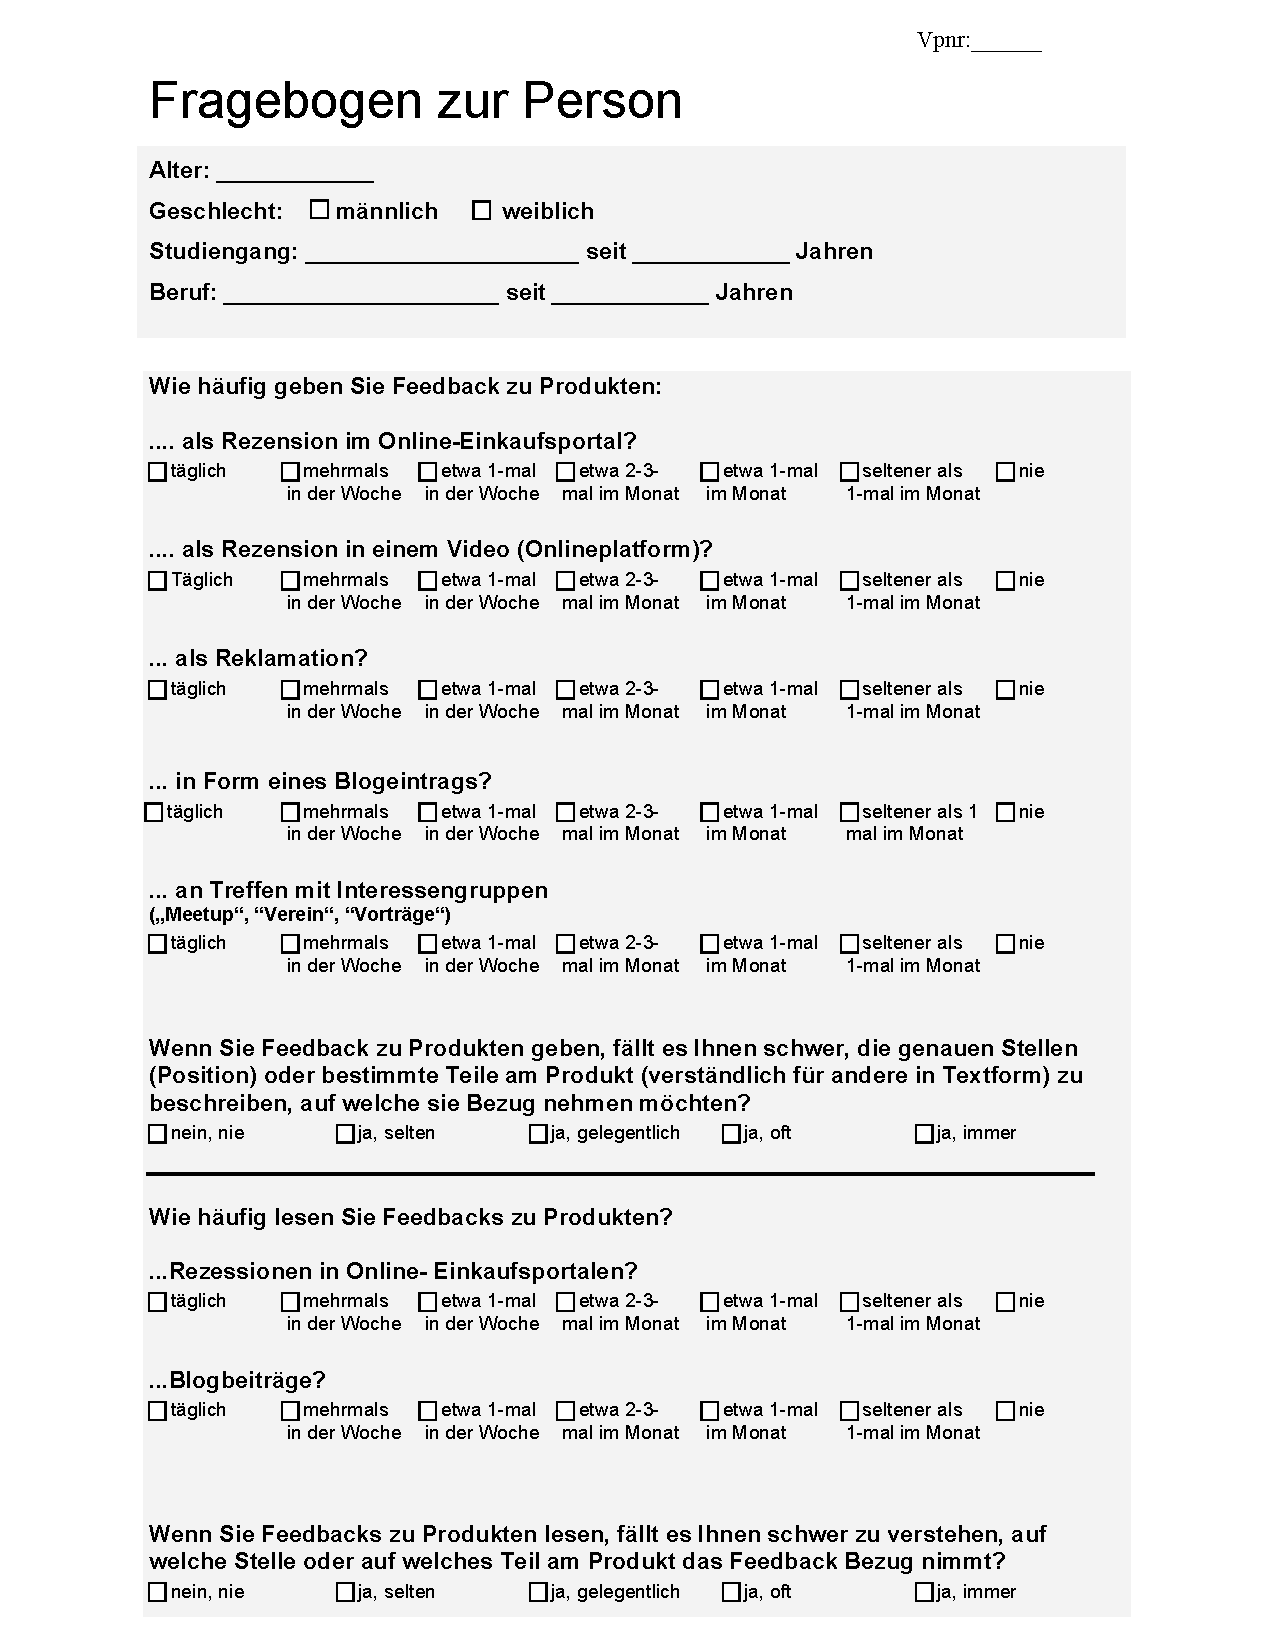
\includepdf[pages=-]{resources/anhang/Demografischer_Fragebogen.pdf}

